% THIS IS SIGPROC-SP.TEX - VERSION 3.1
% WORKS WITH V3.2SP OF ACM_PROC_ARTICLE-SP.CLS
% APRIL 2009
%
% It is an example file showing how to use the 'acm_proc_article-sp.cls' V3.2SP
% LaTeX2e document class file for Conference Proceedings submissions.
% ----------------------------------------------------------------------------------------------------------------
% This .tex file (and associated .cls V3.2SP) *DOES NOT* produce:
%       1) The Permission Statement
%       2) The Conference (location) Info information
%       3) The Copyright Line with ACM data
%       4) Page numbering
% ---------------------------------------------------------------------------------------------------------------
% It is an example which *does* use the .bib file (from which the .bbl file
% is produced).
% REMEMBER HOWEVER: After having produced the .bbl file,
% and prior to final submission,
% you need to 'insert'  your .bbl file into your source .tex file so as to provide
% ONE 'self-contained' source file.
%
% Questions regarding SIGS should be sent to
% Adrienne Griscti ---> griscti@acm.org
%
% Questions/suggestions regarding the guidelines, .tex and .cls files, etc. to
% Gerald Murray ---> murray@hq.acm.org
%
% For tracking purposes - this is V3.1SP - APRIL 2009

\documentclass{acm_proc_article-sp}

\usepackage[utf8]{inputenc}
\usepackage{graphicx}
\usepackage{caption}

\begin{document}

\title{Rapport Matlab : Simulation d'une chaîne de transmission numérique sur canal gaussien à bande limitée}

%\subtitle{[Extended Abstract]
%\titlenote{A full version of this paper is available as
%\textit{Author's Guide to Preparing ACM SIG Proceedings Using
%\LaTeX$2_\epsilon$\ and BibTeX} at
%\texttt{www.acm.org/eaddress.htm}}}

%
% You need the command \numberofauthors to handle the 'placement
% and alignment' of the authors beneath the title.
%
% For aesthetic reasons, we recommend 'three authors at a time'
% i.e. three 'name/affiliation blocks' be placed beneath the title.
%
% NOTE: You are NOT restricted in how many 'rows' of
% "name/affiliations" may appear. We just ask that you restrict
% the number of 'columns' to three.
%
% Because of the available 'opening page real-estate'
% we ask you to refrain from putting more than six authors
% (two rows with three columns) beneath the article title.
% More than six makes the first-page appear very cluttered indeed.
%
% Use the \alignauthor commands to handle the names
% and affiliations for an 'aesthetic maximum' of six authors.
% Add names, affiliations, addresses for
% the seventh etc. author(s) as the argument for the
% \additionalauthors command.
% These 'additional authors' will be output/set for you
% without further effort on your part as the last section in
% the body of your article BEFORE References or any Appendices.

\numberofauthors{2} %  in this sample file, there are a *total*
% of EIGHT authors. SIX appear on the 'first-page' (for formatting
% reasons) and the remaining two appear in the \additionalauthors section.
%
\author{
% You can go ahead and credit any number of authors here,
% e.g. one 'row of three' or two rows (consisting of one row of three
% and a second row of one, two or three).
%
% The command \alignauthor (no curly braces needed) should
% precede each author name, affiliation/snail-mail address and
% e-mail address. Additionally, tag each line of
% affiliation/address with \affaddr, and tag the
% e-mail address with \email.
%
% 1st. author
\alignauthor
Hoël Boëdec\\
       \affaddr{ENSIMAG - ISSC}\\
       \affaddr{3 rue Amiral Courbet}\\
       \affaddr{Grenoble, France}\\
       \email{hoel.boedec@phelma.grenoble-inp.fr}
% 2nd. author
\alignauthor
Fournier Mickaël\\
       \affaddr{ENSIMAG - ISSC}\\
       \affaddr{22 rue Francis Jaquard}\\
       \affaddr{Grenoble, France}\\
       \email{mickael.fournier@phelma.grenoble-inp.fr}
}
% There's nothing stopping you putting the seventh, eighth, etc.
% author on the opening page (as the 'third row') but we ask,
% for aesthetic reasons that you place these 'additional authors'
% in the \additional authors block, viz.
% \additionalauthors{Additional authors: John Smith (The Th{\o}rv{\"a}ld Group,
% email: {\texttt{jsmith@affiliation.org}}) and Julius P.~Kumquat
% (The Kumquat Consortium, email: {\texttt{jpkumquat@consortium.net}}).}
% \date{30 July 1999}
% Just remember to make sure that the TOTAL number of authors
% is the number that will appear on the first page PLUS the
% number that will appear in the \additionalauthors section.

\maketitle
\begin{abstract}
    
\end{abstract}

\section{Introduction}

\begin{figure}
\centering
\epsfig{file=Alice&Bob.eps, height=2in, width=4in}
\end{figure}

\begin{figure}
\centering
\epsfig{file=Steganography_original.eps, height=1in, width=1in}
\caption{[Wikipedia] Image d'un arbre avec une image steganographiquement cachée. La photo cachée est révélée en ne gardant que les deux bits de poids faible de chaque couleur qui la compose. L'image cachée est visible ci-dessous.}
\end{figure}

\begin{figure}
\centering
\epsfig{file=Steganography_recovered.eps, height=1in, width=1in}
\caption{[Wikipedia] Image d'un chat extraite de l'image d'arbre ci-dessus.}
\end{figure}

\begin{center}
\includegraphics[height=3cm]{DirtyConstellation.eps}
\end{center}

\begin{figure}
\centering
\epsfig{file=Alice&Bob2.eps, height=2in, width=3in}
\end{figure}



\section{Génération aléatoire des éléments binaires}


\section{Conversion des éléments binaires en symboles (mapping)}


\section{Conversion numérique - analogique}
\subsection{Expansion}
\subsection{Etude des filtres}
\subsection{Mise en forme des symboles}


\section{Ajout du bruit blanc gaussien}


\section{Conversion analogique - numérique}
\subsection{Filtrage adapté}
\subsection{Décimation}


\section{Prise de décision (demapping)}


\section{Calcul du taux d'erreur binaire}


\section{Mesures de performances}


\section{Optionnel}
\subsection{Autres impulsions de mise en forme}
\subsection{Rapport signal à bruit sur la variable de décision}
\subsection{Analyseur de spectre}


\section{Conclusion}

\balancecolumns
% That's all folks!
\end{document}
